\documentclass{article}
\usepackage{amssymb}
\usepackage{graphics}
\usepackage{amsthm}

\usepackage{epsfig}
\begin{document}

\section{Threat model and analysis}

\subsection{General setup}

We consider the case where the app may be malicious and trying to
pinpoint the user's location at a given point in time, under the case
that the user potentially travels along a certain path.  Therefore, we
are attempting to minimize the knowledge that an attacker has about a
user at any individual point in time, under the constraint that the
user needs to have some utility in the app.

% Jeff, I think I get overzealous about italics, apologies.

We assume that there is some underlying space, $M$, called the
\emph{map}, in which the user's true position $p_i$ lies, where $p$ is
indexed by time $i$.  We assume that user will present their points to
the attacker by presenting their location within the \emph{skew set}
$M' \subseteq M$.  The user can guarentee their location security
because it associates each true position $p_i \in M$ with a skewed
position $p'_i \in M'$.  The user is assumed to have some \emph{skew
  function} which skews their location: $h : M \rightarrow M'$.  The
attacker $\mathcal{A}$ is attempting to invert $h$ to produce
$h^{-1}$.

To aid the user in skewing their values, we introduce a set of
\emph{regions}: each point $p \in M'$ will be associated with a subset
of $M$, $\mathcal{R}_p \subseteq M$ and is called the skew region of
$p$.  In the standard location truncation model, fuzzing corresponds
to selecting these $\mathcal{R}_p$ to correspond to square regions
around points in the area, but we provide a counterexample as to why
this can lead to an attacker precisely obtaining $p_i$ (along a
certain path).  Note that while we typically assume that each
$\mathcal{R}_p$ is disjoint, this need not necessarily be the case.
\\

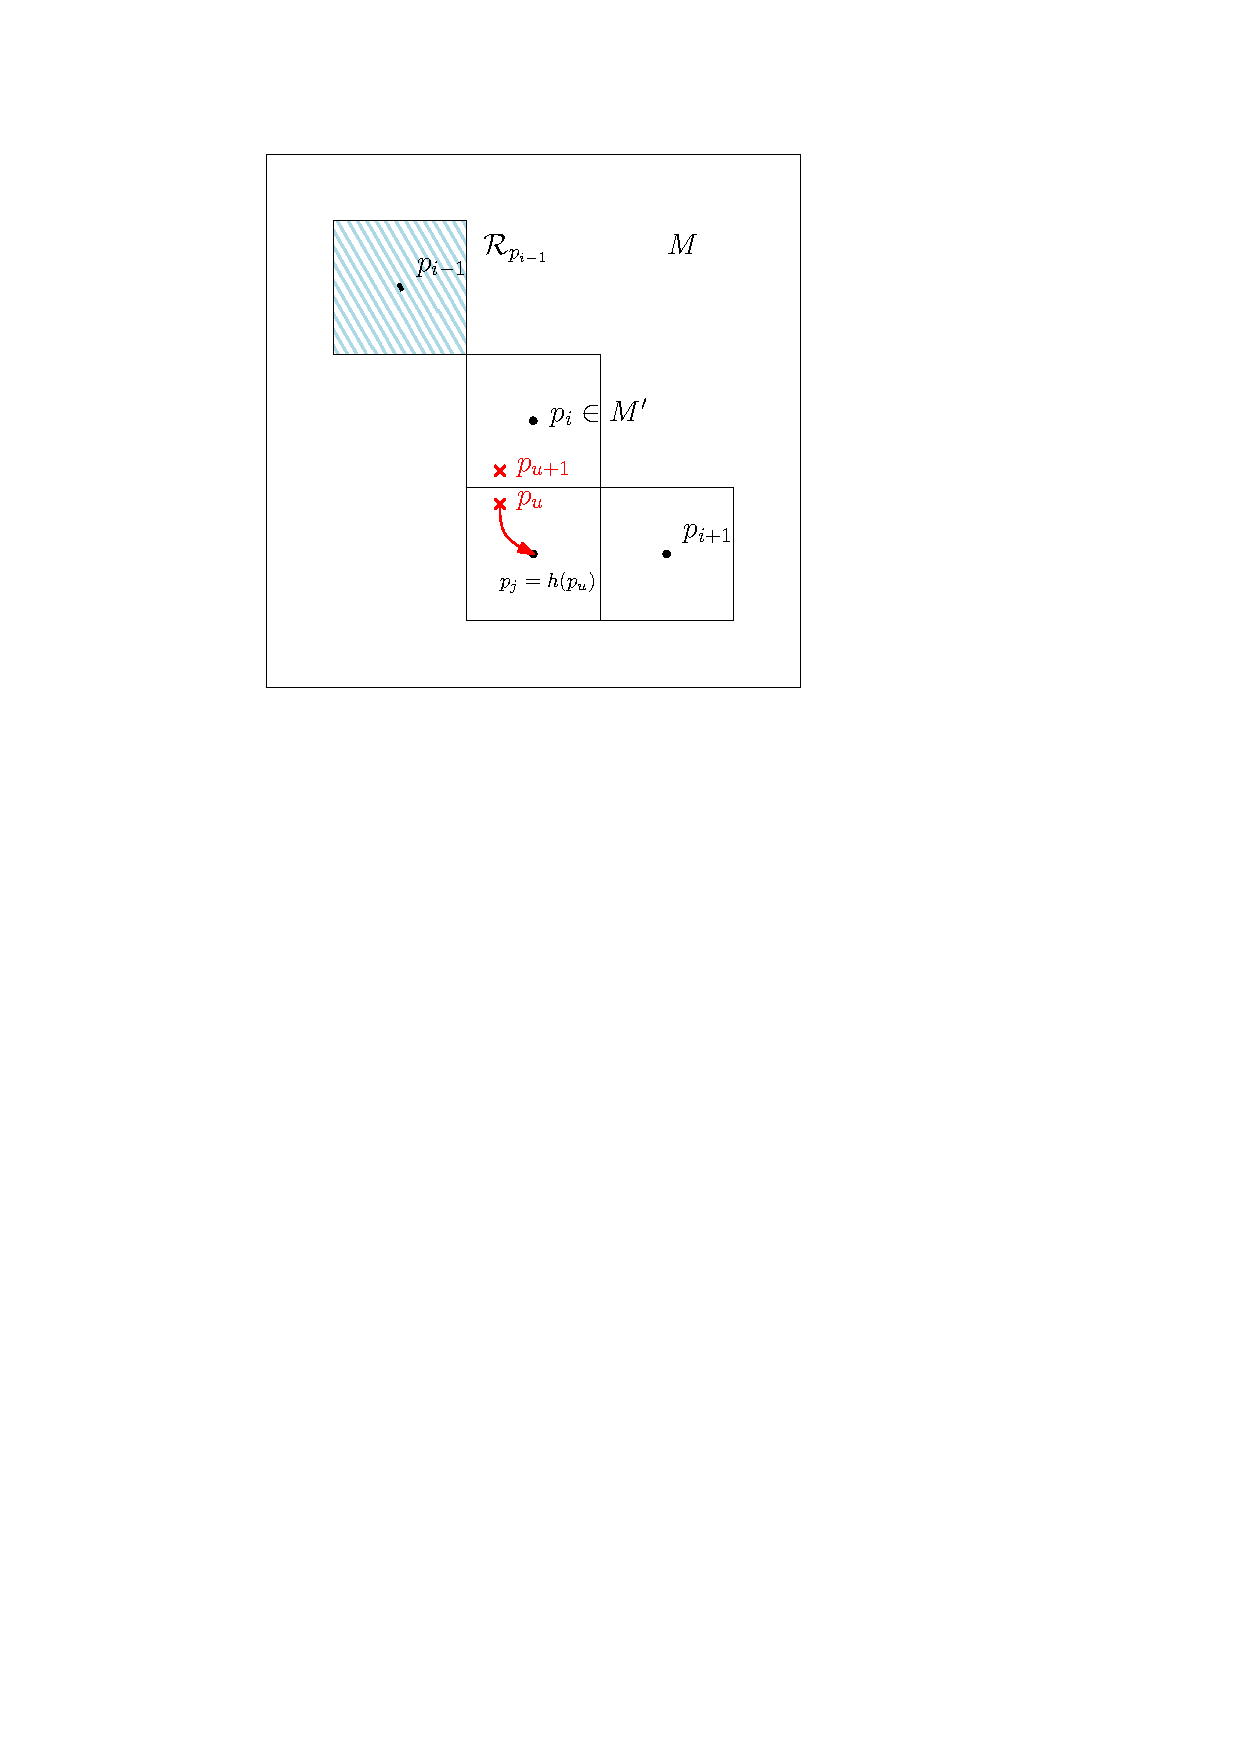
\includegraphics{threat_model_image.pdf}

\subsection{Location query games}

We assume an adversarial attacker $\mathcal{A}$, which is attempting
to discover the user's true position at an arbitrary time $p_i$.  In
using the location based service, the user will produce \emph{queries}
consisting of their presented location ($\in M'$), and the adversary
will reply with answers within the \emph{answer set} $\Gamma$.  For
any given app, the answer set $\Gamma$ will consist of location
targeted information (such as lists of the nearest hospitals or gas
stations).  The user $\mathcal{U}$ and adversary $\mathcal{A}$
interact via a discrete set of moves, at each step $i$, $\mathcal{U}$
sends $\mathcal{A}$ their presented position $p_i$, and $\mathcal{A}$
sends a response within the answer set, $r(p_i) = \gamma_i \in Gamma$.
Through the game, $\mathcal{A}$ can learn only the set of queries
which $\mathcal{U}$ has made, $\langle p_i | i \in \{0,\dots,n\}
\rangle$.  $\mathcal{A}$ models their estimation of $\mathcal{U}$'s
position at time $i$ by a probability distribution: $\mathrm{Pr}(p_i =
x \in M)$.

We assume that the user has some utility function $u : \Gamma \times
\Gamma \rightarrow [0,1]$, which gives the utility of the skewed
answer.  For example, if $\gamma_0$ is the user's \emph{true}
location, and $\gamma_1 = h(p_i)$ is the user's presented location,
then $u(\gamma_0,\gamma_1)$ will give a measure of \emph{how much} the
skewed location hurts the user.  Here we posit the existence of the
utility function to the user, in reality it must be sensibly picked
(we present techniques to do so later in the paper).  We point two
edge cases: $u(\gamma_0,\gamma_1) = 1$ is the case where the user can
arbitrarily lie about their location without harm.  For example, the
app may present an ad to the user targeted to their location.  If the
app only uses location for presenting targeted ads, and the user does
not care about these ads, it may be sensible for this to be the
utility function.  

\newtheorem{noinformation}{Best case scenario for single poll} 

If the attacker observes only a single point, they can only learn
location to within a certain delta.

\subsection{Single Dimension Case}

\begin{figure}[h]
  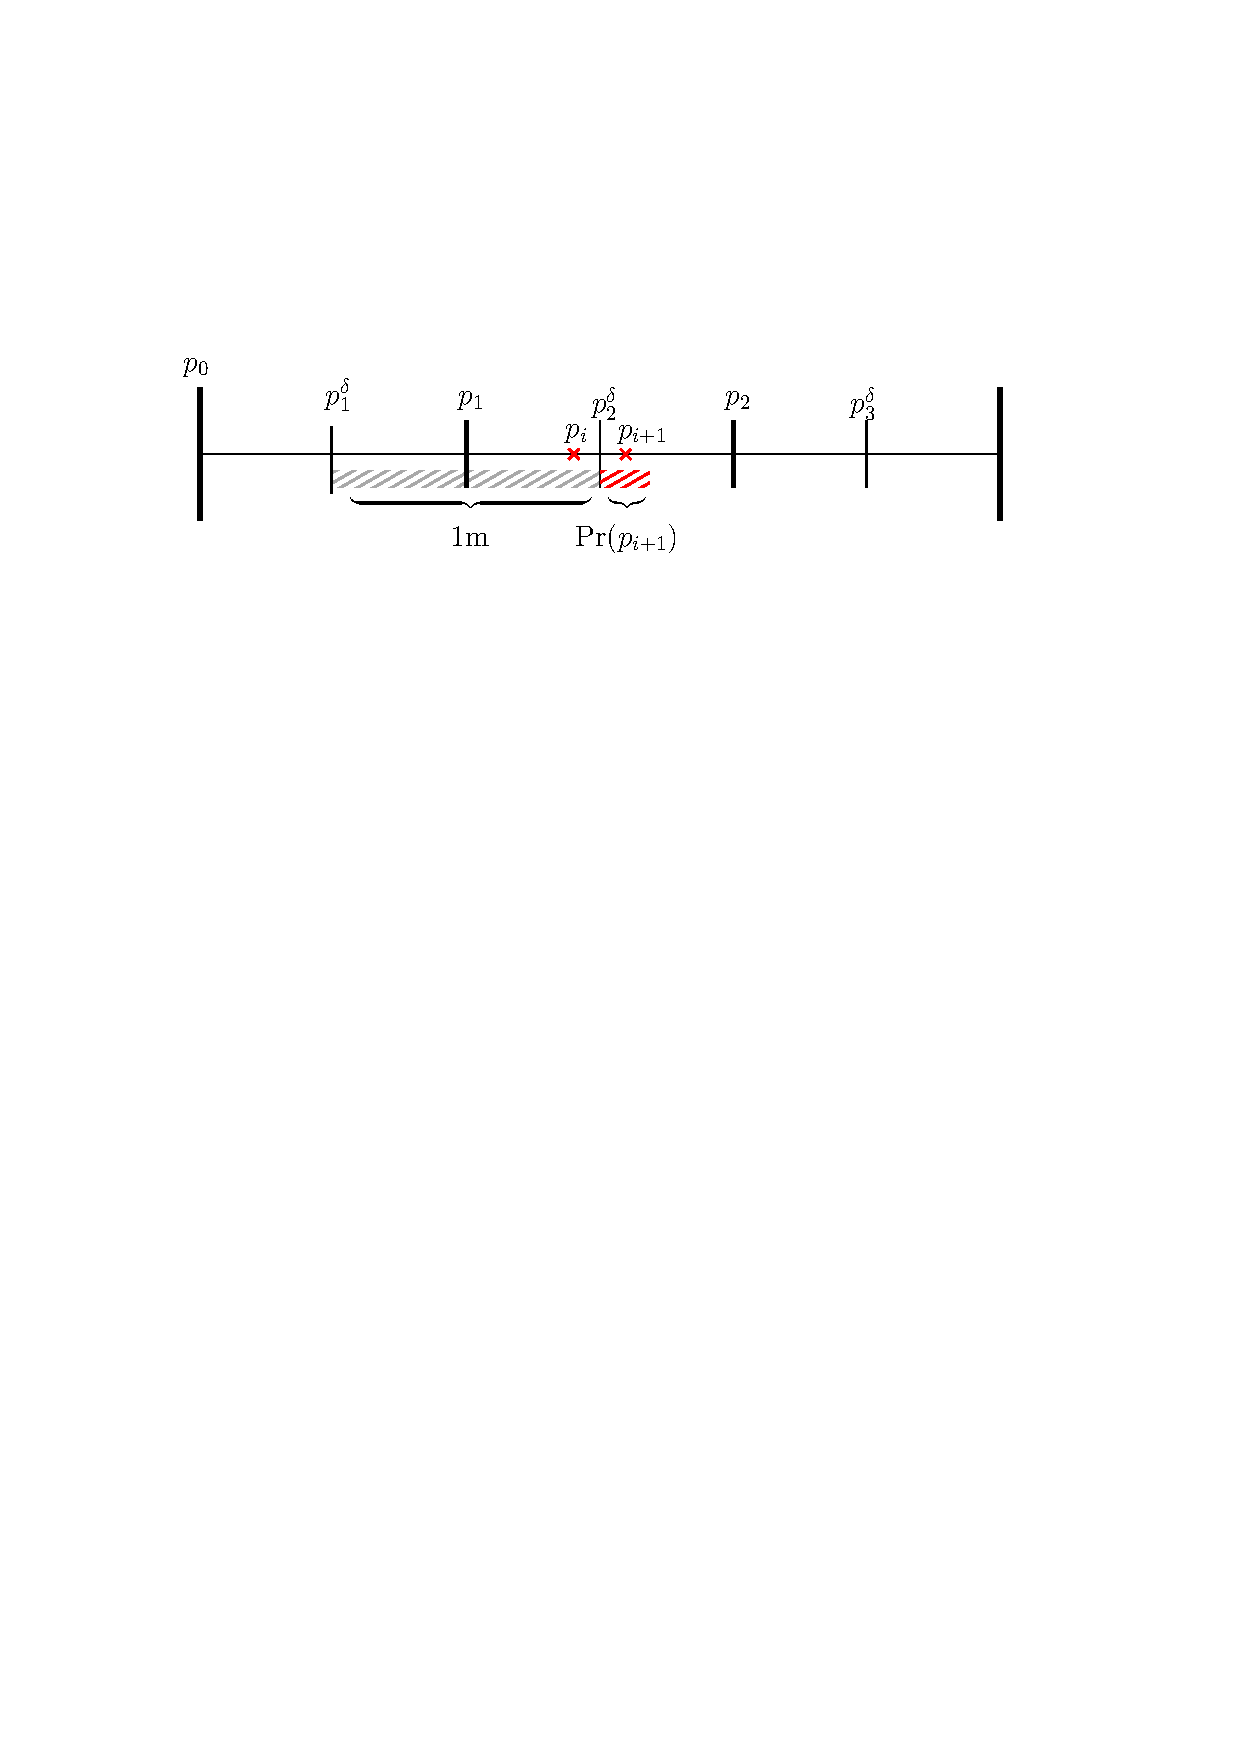
\includegraphics[width=\textwidth]{threat_model_diagram_truncation_bad.pdf}
  \caption{Location model with truncation, we assume $\mathcal{U}$
    begins at position $p_i$ and proceeds to $p_{i+1}$ in a step, thus
    revealing their location.}
\end{figure}

In the simplest case, we consider the game in one dimension.  We
assume that the user is fuzzing their location using a truncation
based fuzzing technique.  In this case, the regions are 1 meter in
area (arbitrarily), and each ``point'' $p_i$ occurs on the meter.  We
assume that the attacker can take advantage of successive rounds to
model the user's location, and that the user makes requests with
period $\delta_r = 1 s$, and that the user travels at $s = .1
\frac{\textrm{m}}{\textrm{s}}$.

\paragraph{Simple Truncation and Associated Problems}

Consider that the attacker $\mathcal{A}$ starts observing
$\mathcal{U}$ at time $i$, as $\mathcal{U}$ makes a request to receive
data based on point $p_1$.  If $\mathcal{A}$ has only the knowledge of
the point $p_i$, it is impossible for the attacker to know
$\mathcal{U}$'s to any better a precision than 1 meter.  (Proof here.)
However, if the user presents their location at $p_1$, and then
successively presents their location at $p_2$, the attacker
immediately knows that their location must be somewhere in the range
$[p_2^{\delta},p_2^{\delta} + \delta_r\, s] = [\frac{p_2 + p_1}{2},
\frac{p_2 + p_1}{2} + .1]$.  This is because, in the worst case
scenario, $p_i$ could have been at $\frac{p_2 + p_1}{2} - \delta$, and
if the user was traveling at full speed for the duration of the
polling period, they would subsequently be at $\frac{p_2 + p_1}{2} +
.1$.  Assuming that the user travels at a constant speed, their
location can now be pinpointed with high accuracy.  (And with
successive rounds, the attacker can increase their estimate as to the
user's location.)

(Jeff, what do we do about the realistic fact that user's change their
speed, stop and start over time, etc...?, that seems to be a fairly
integral part of this construction.)

(Jeff: if the user does not hold constant speed, they eventually
recover their privacy, and can arbitrarily wander around.  The only
time their location is really in danger is right after they cross the
line...)

\paragraph{Randomized Truncation}

\begin{figure}[h]
  \label{fig:randgrid}
  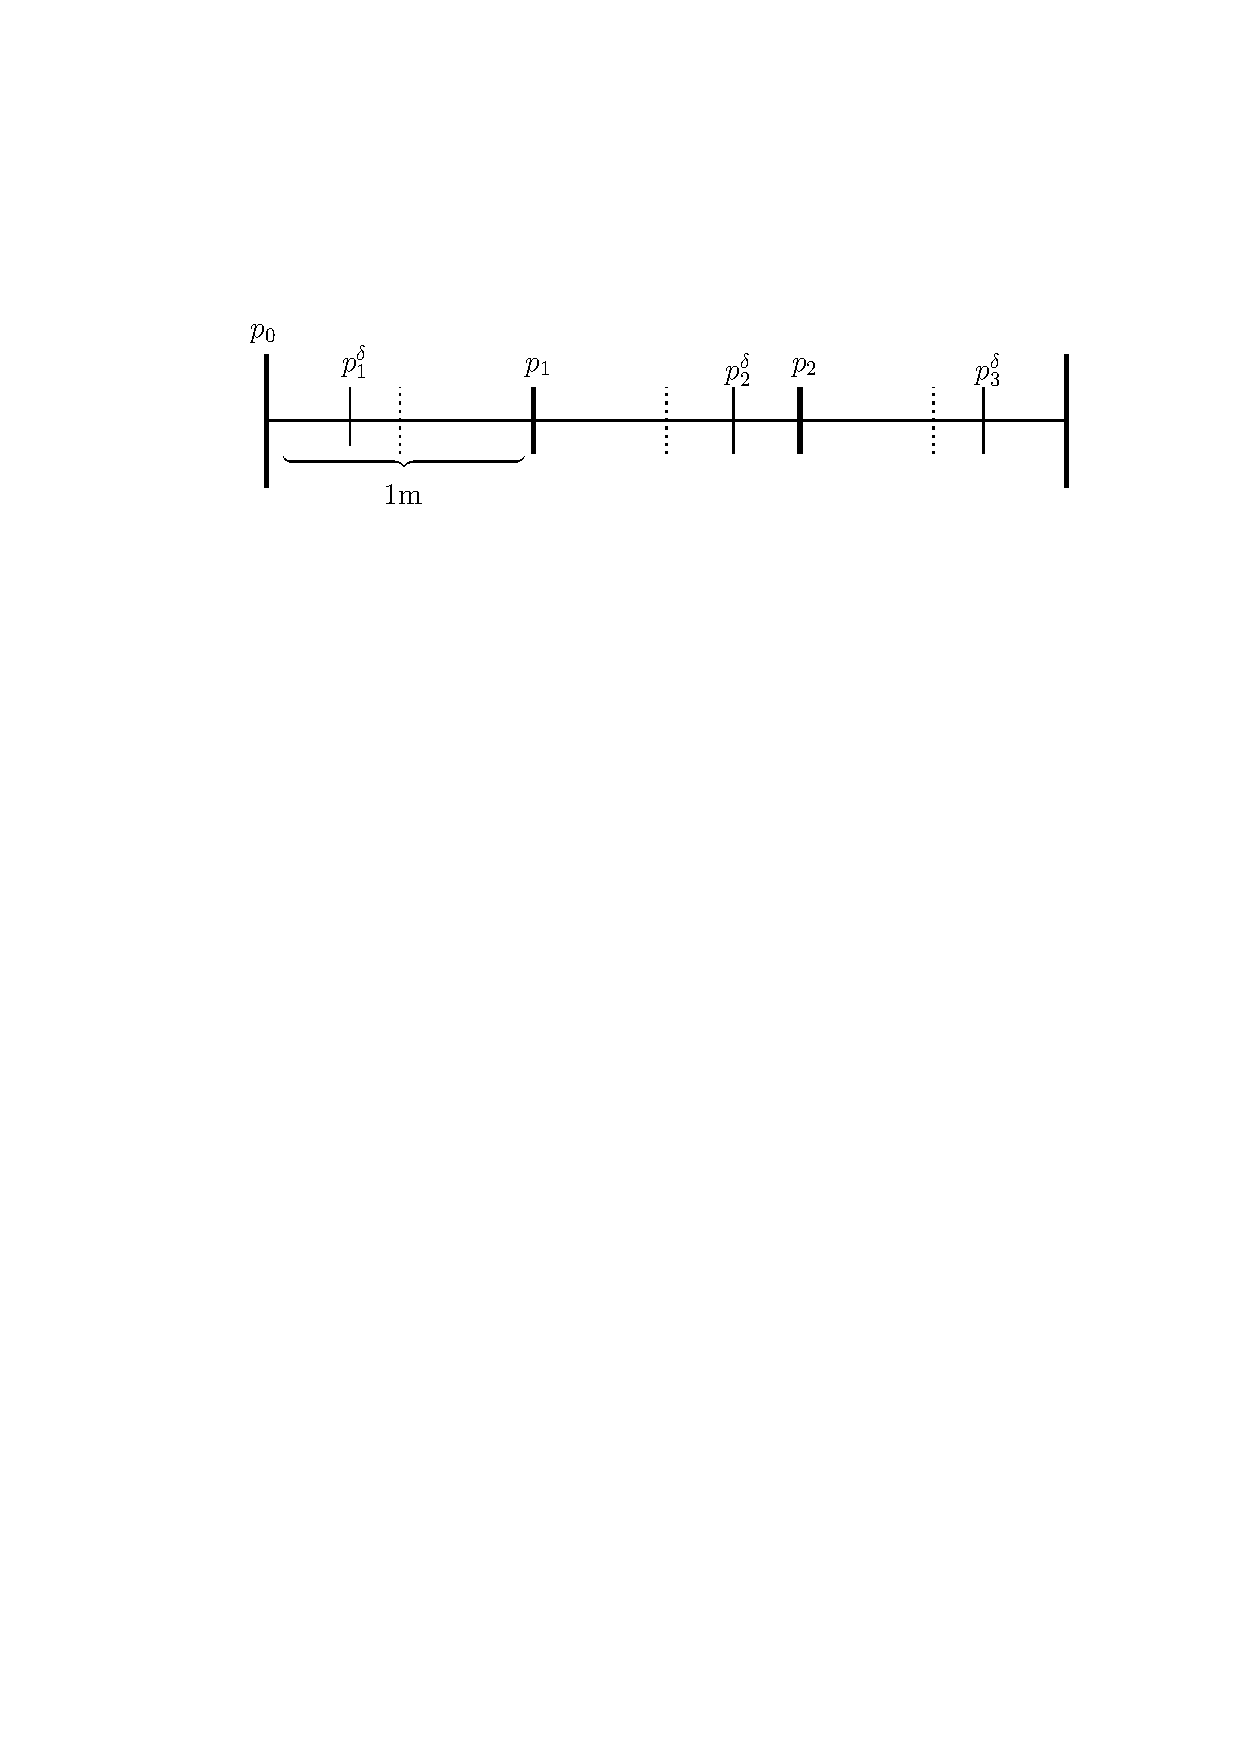
\includegraphics[width=\textwidth]{threat_model_diagram_randomized_truncation.pdf}
  \caption{In the case of randomized location, we continue to use a
    grid with discrete points, but we randomly pick the ``crossover''
    points.}
\end{figure}

Because the truncation based model allows the user's location to be
precisely targeted, we consider a different model.  Intuitively, the
problem introduced in the truncation based model is due to the fact
that (assuming some bound on the user's speed) the user can use the
known cutoff points to ``pin'' the user within some range (out of
which they could not travel quickly).  Using this idea, one potential
idea might be to randomize the ``cutoff'' points.  Instead of choosing
the crossover point between $p_i$ and $p_{i+1}$ (which we call
$p_i^{\delta}$ to be $\frac{p_i+p_{i+1}}{2}$, we can choose it to be
some random point in the range $(p_i,p_{i+1})$.

In this section we consider the concrete case of a ``crossover point''
being chosen uniformly randomly in the range $(p_i,p_{i+1})$ (note
that in our truncation based scenario, $p_{i+1} - p_i$ is a constant).
We give an example in \ref{fig:randgrid}: $p_1$ and $p_2$ are points,
and each $p_i^{\delta}$ (the crossover points) are chosen randomly
uniformly between each two actual grid markers.  (We have also drawn
the original crossover lines from the previous section.)

We show that if the user is traveling at a known constant speed, this
method will allow the attacker to model the user's location (to an
arbitrary confidence interval) after a number of rounds depending on
$\delta_u$: the maximum distance away from the actual location at
which the user is willing to present themselves.  First consider the
case where $\mathcal{U}$ is traveling at a constant speed and is
continuously querying $\mathcal{A}$.  Consider the case of a
randomized grid (where the crossover points are chosen as in the
previous paragraph), the important point to note is that, whenever a
user successively polls an adversary they implicitly give away their
location 

\begin{figure}[h]
  \label{fig:interarrival}
  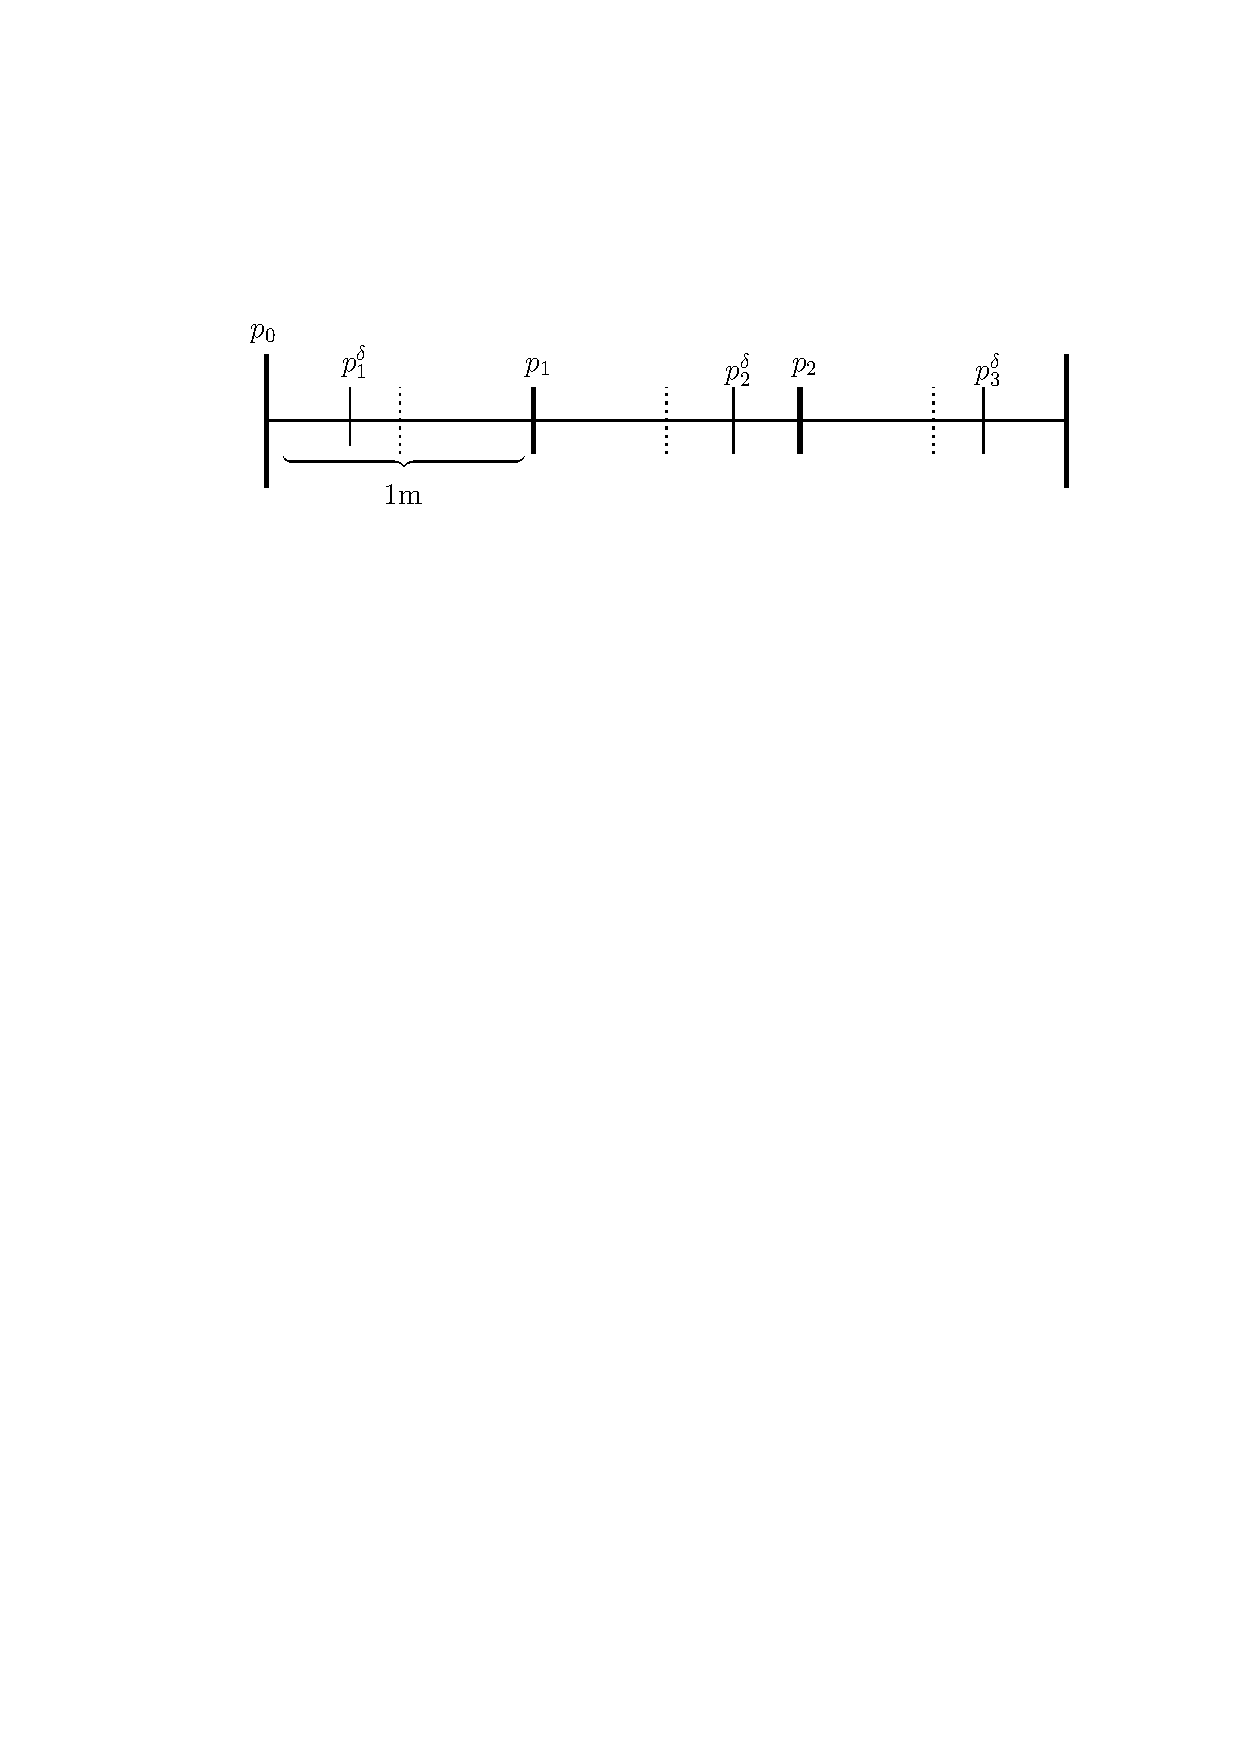
\includegraphics[width=\textwidth]{threat_model_diagram_randomized_truncation.pdf}
  \caption{If the user polls their location at intervals quickly
    enough they will implicitly reveal their location to the
    adversary.}
\end{figure}

Consider Figure \ref{fig:interarrival}.  If we assume that queries are
made at a near continuous rate, the user will implicitly reveal the
length $p_2^{\delta}-p_1^{\delta}$, as they are traveling at constant
speed.  If $\mathcal{A}$ continues to monitor these crossover
intervals, they can precisely estimate the total accumulated distance
and then use this to solve for the initial point $p_0$.

Jeff, informally I've figured out this: if you continue to look at
queries in the continuous case, you can precisely estimate the ``total
length'' you've accumulated so far.  After you get a long enough total
length you can start using this, along with your assumption about the
user's utility (they will never choose a point more than 1 meter
away), to solve for the initial point $p_0$.  I feel fairly confident
that if I write out and grind the equations I can characterize how
long it will take the adversary to learn the initial point.

So next, I wondered, if the problem is that we're polling a continuous
rate, perhaps we should be slower, and poll at a discrete rate.  I did
a few examples and realized that while this slows convergence, it sort
of reduces to the original case.  In fact, it exactly reduces to the
previous case if you take your ``utility bound'' --- the maximum
distance you're allowed to vary from ground truth --- to tack a
$\delta_s$ term on, where $\delta_s$ is the maximum distance
accumulated in the interquery time.

I then played around with the idea of only querying the server when
you knew you crossed the threshold.  But it turns that if the
adversary knows this then not querying also reveals information!

It seems that everything I do sort of reduces to this case of the user
($\mathcal{U}$) having a maximum error, and this parameterizes the
rate at which the adversary learns your location.

But this is all in the case of a constant rate of speed!  In reality
we will probably not have a constant rate of speed: how do you think
that plays into it?  If you do not have a constant speed, this
``random grid'' method does have an advantage over the previous
method: the adversary can't instantaneously target you as you cross
the line.  Since in reality your speed will fall under some
distribution, your location privacy generally increases over time
after you've crossed the line into the ``safe zone.''

And then I sort of worry about how this stacks up to the other
location based privacy papers I've recently found: the analysis I'm
doing is all very ``napkin''-y, where theirs seems much more reasoned
and game theoretic.

%% \subsection{Generalizing to two dimensional spaces}

\end{document}
